\chapter{Desarrollo: Iteración III} % Main chapter title

\label{Chapter8} % Change X to a consecutive number; for referencing this chapter elsewhere, use \ref{ChapterX}

\steveCabecera{Capítulo 8. \emph{Iteración III}} % Change X to a consecutive number; this is for the header on each page - perhaps a shortened title

%----------------------------------------------------------------------------------------
%	SECTION 1
%----------------------------------------------------------------------------------------
\section{Introducción}
En este capítulo se documentan aspectos relevantes relacionados con la codificación que se realizó en la tercera iteración de desarrollo del software.\\
Aparece un nuevo requerimiento funcional a partir de la devolución de un grupo de early testers quienes solicitaron un modo de accionamiento rápido a través de alguna interfaz en la pantalla de bloqueo de android.
Quizás el cambio más importante introducido en esta iteración es la inclusión del canal de comunicación con los módulos a través de internet. Se describirá el modo de empleo del protocolo MQTT para conseguir la ejecución de los RPC. Se codificó un wrapper reactivo sobre la librería paho de eclipse empleada para configurar el cliente MQTT y su posterior empleo en la aplicación. %%Request Response over Subscribe Queues, message duplicaction,message payload format
Dado que se habilitó un nuevo canal, el repositorio deberá decidir cuando ejecutar los RPC por LAN o Internet, se expondrá el algoritmo utilizado para la selección de los canales.
Finalmente así como se hizo para las iteraciones previas se expondrán las implementaciones más interesantes de la lógica de negocios de los caso de uso planificados para esta iteración.
%% implementaion sofisticada con templates genericos
\section{Accionamiento Rápido}
Luego de producir las primeras unidades del módulo
decidimos distribuirlas a un grupo de usuarios que estaban interesados en probar el producto.
Pasado el período de pruebas nos pusimos en contacto con ellos y tomamos registro de sus devoluciones.
Un comentario común entre la mayoría fue que les parecía que tenían que hacer demasiado para accionar sus portones.
Apareció entonces la propuesta de adicionar un elemento visual en la pantalla de bloqueo de android
que permita el accionamiento sin tener que desbloquear el teléfono.

En la figura ~\ref{fig:notif_design} se puede ver una maqueta de cómo luciría el control rápido implementado como una notificación permanente de android.

Como medidas de seguridad para evitar accionamientos accidentales se propuso limitar los módulos
disponibles para este tipo de accionamiento a aquellos que se encuentren dentro de un radio de 320 metros alrededor del teléfono. También se incluyó un segundo botón que habilita el accionado, obligando al usuario a realizar 2 movimientos voluntarios para completar la acción: tomando como referencia la figura ~\ref{fig:notif_design} será necesario presionar el botón (3) y luego el botón (4).


\begin{figure}[htbp]
	\centering
	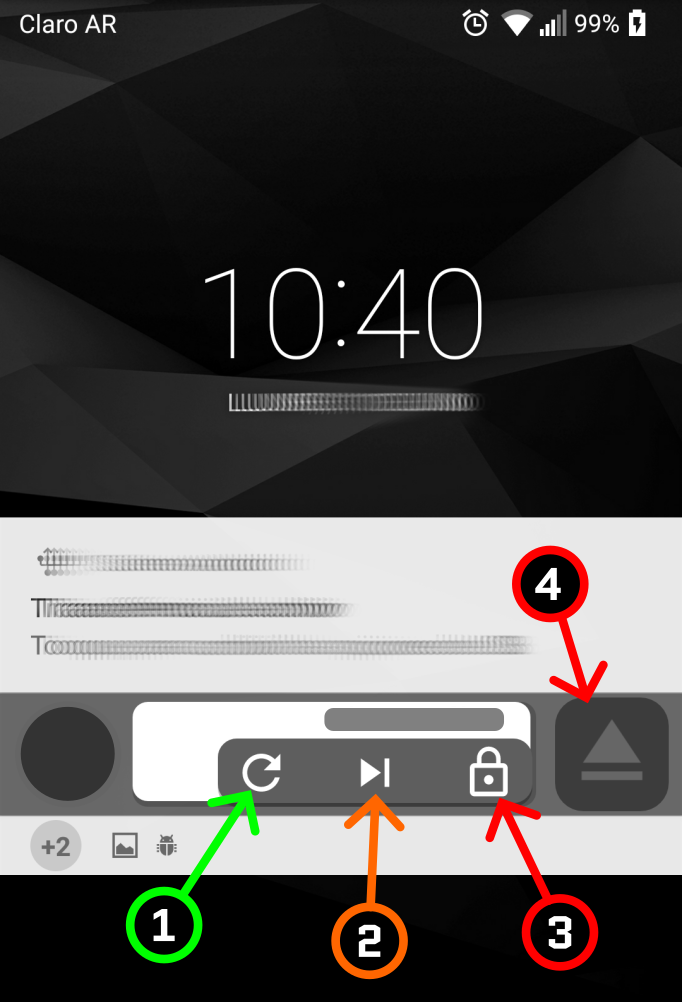
\includegraphics[width=0.4\textwidth]{Figures/iter3/module_notif.png}
	\rule{35em}{1pt}
	\caption[Wireframe]{Maqueta de diseño de la notificación permanente para el control rápido. (1) Botón para buscar los módulos disponibles, (2) Botón para rotar el módulo seleccionado, (3) Botón para habilitar el accionamiento, (4) Botón para accionar el módulo seleccionado.}
	\label{fig:notif_design}
\end{figure}

\section{Canal de comunicación por Internet}
Uno de los aspectos más sobresalientes de la propuesta de valor del producto es la posibilidad
de monitorear, configurar y accionar el módulo de manera remota a través de internet.
En la figura ~\ref{fig:comunic_mod_app} se muestra el esquema de conexión para el modo de operación por internet.
\subsection{Broker MQTT}
Para poder usar el protocolo es necesario contar con un servidor que provea las funciones del broker MQTT.\\
Existen muchas implementaciones listas para usar incluso de código abierto y que se ofrecen de manera gratuita en la red.
De las más populares se optó por un producto chino de nombre \textbf{EMQX}, se trata de una implementación completa del broker MQTT
más un tablero de control y monitoreo web accesible a través del navegador. 
Los autores ofrecen una imagen docker lista para configurar y montar sobre contenedores.
Adicionalmente cuenta con una API HTTP que permite la gestión de tópicos, clientes, sesiones, políticas de acceso y más. Esta implementación también admite el escalado horizontal mediante la configuración de clusters de brokers, estas funcionalidades avanzadas quedan fuera del alcance del presente proyecto.

Para la primera versión del producto se configuró un contenedor de broker EMQX en un servidor virtual privado.
Actualmente EMQX Cloud ofrece un servicio a demanda que no requiere de contar con infraestructura propia.

\subsection{Adaptación del protocolo MQTT}
Como se mencionó en la sección ~\ref{section:mqtt} el protocolo MQTT implementa el patrón de arquitectura Publish-Subscribe .
Sin embargo por definición ~\ref{section:rpc} el protocolo RPC depende de la implementación del patrón Request-Response entre cliente y servidor. 
%sin embargo está claro que la ejecución de protocolos RPC necesita de un canal de comunicación que admita  Request-Response...

Esta controversia se resuelve del lado de la aplicación ofreciendo una adaptación sobre el protocolo MQTT.
Es decir, la suscripción a los tópicos, el envío de mensajes y el formato de los mismos se realizará de manera tal que el modo de comunicación entre aplicación y módulos permita la correcta ejecución de los RPC.

\subsubsection{Formato del Mensaje}
Los mensajes se envían en el payload del paquete MQTT y conservan los formatos descritos para las solicitudes y respuestas descritas en la sección ~\ref{section:rpc} pero para admitir la adaptación necesaria se agregan tres campos extra a saber:
\begin{itemize}
	\item Requester: Es el identificador único del usuario que intenta ejecutar el RPC. Será utilizado por el módulo para autorizar la operación y no se incluye en la respuesta.
	\item Tag: Es la concatenación de los identificadores del módulo y el usuario ejecutor. Este campo se copia sin alterar en la respuesta. Permite a la aplicación identificar el origen de la respuesta.
	\item Id: Es el identificador único del mensaje. Es un número aleatorio que genera la aplicación para cada mensaje con el propósito de detectar duplicados.
\end{itemize}

\begin{multicols}{3} % Change 3 to desired number of columns
	
	% Your content for column 1
	{\small Solicitudes por MQTT:}
	\begin{lstlisting}
{
  "id": 103,
  "method": "method_name",
  "params":{
  "un_parametro": ...,
  "otro_parametro": ...,
  ...
  }

  "requester": 3514123456,
  "tag": "urbit_777::3514123456",
  "id": 2356897
}
	\end{lstlisting}
	
	\columnbreak % Insert a column break between columns
	
	% Your content for column 2
	{\small Respuestas exitosas por MQTT:}
	\begin{lstlisting}
{
  "id": 103,
  "result":{
  "un_resultado": ...,
  "otro_resultado": ...,
  ...
  }
  "tag": "urbit_777::3514123456",
  "id": 2356897
}
	
	\end{lstlisting}
	
	\columnbreak % Insert a column break between columns
	
	% Your content for column 3
	{\small Respuestas con error por MQTT:}
	\begin{lstlisting}
{
  "id": 103,
  "error":{
  "code": 404,
  "message": "... no existe",
  ...
  }
  "tag": "urbit_777::3514123456",
  "id": 2356897
}
	
	\end{lstlisting}
	
\end{multicols}

\subsubsection{Tópicos y Suscripciones}
\textbf{EJECUCIÓN RPC}

Todos los módulos conectados al Broker MQTT estarán suscritos a un único tópico con el siguiente formato:
\textbf{\texttt{urbit-??????/request}}\\
Los signos de interrogación corresponden al UID de cada módulo. En este tópico recibirá las solicitudes de ejecución de RPC.

Al mismo tiempo publicarán las respuestas a los tópicos generados para cada usuario que respetan el siguiente formato:\\
\textbf{\texttt{urbit-??????/response/XXXXXXXXXX}}\\
Los signos de interrogación corresponden al UID de cada módulo y las equis al UID del usuario. En este tópico se publican las respuestas a las solicitudes de ejecución de RPC.

Los módulos publicarán los cambios en el estado de apertura a el tópico con el siguiente formato.
\textbf{\texttt{urbit-??????/status}}\\

\textbf{INVITACIONES}

Cuando un administrador crea un usuario a partir de su número telefónico en la pantalla de gestión de usuarios. El módulo publica su propio identificador como mensaje retenido en un tópico especial que permite que el usuario invitado pueda encontrar de manera remota este nuevo módulo al que se le a cedido acceso.
Estos tópicos de invitaciones respetan el siguiente formato:\\
\textbf{\texttt{XXXXXXXXXX/invitation/urbit-??????}}\\
Donde las equis corresponden al identificador del usuario invitado y los signos de interrogación al identificador del módulo.

Dado que un usuario puede ser invitado a operar diversos módulos resulta sumamente útil emplear los ``wildcards'' admitidos por MQTT para nombres de tópicos y que permiten suscripciones múltiples. La aplicación cliente se suscribe a un tópico con el siguiente formato:
\textbf{\texttt{XXXXXXXXXX/invitation/+}}\\
Donde las equis corresponden al identificador del usuario y el signo de suma es el comodín que habilitará la recepción de invitaciones de cualquier módulo.

\subsection{RPC sobre MQTT}
Al momento de ejecutar un RPC la aplicación cliente genera el mensaje con el formato indicado anteriormente y lo publica al tópico de solicitudes del módulo. El módulo al recibirlo realizará la tarea de autorización, ejecutará el procedimiento correspondiente y publicará el resultado en el tópico de respuestas.
En la figura ~\ref{fig:act_publish_rpc} se muestra el procedimiento completo de envío de la solicitud de ejecución y la resepción de la respuesta.
El algoritmo puede fallar en 3 escenarios a saber:
\begin{itemize}
	\item Error de conexión al Broker.
	\item Error al momento de Publicar el mensaje.
	\item El timeout fijado para la operación fue excedido sin registrar respuestas.
\end{itemize}

\begin{figure}[htbp]
	\centering
	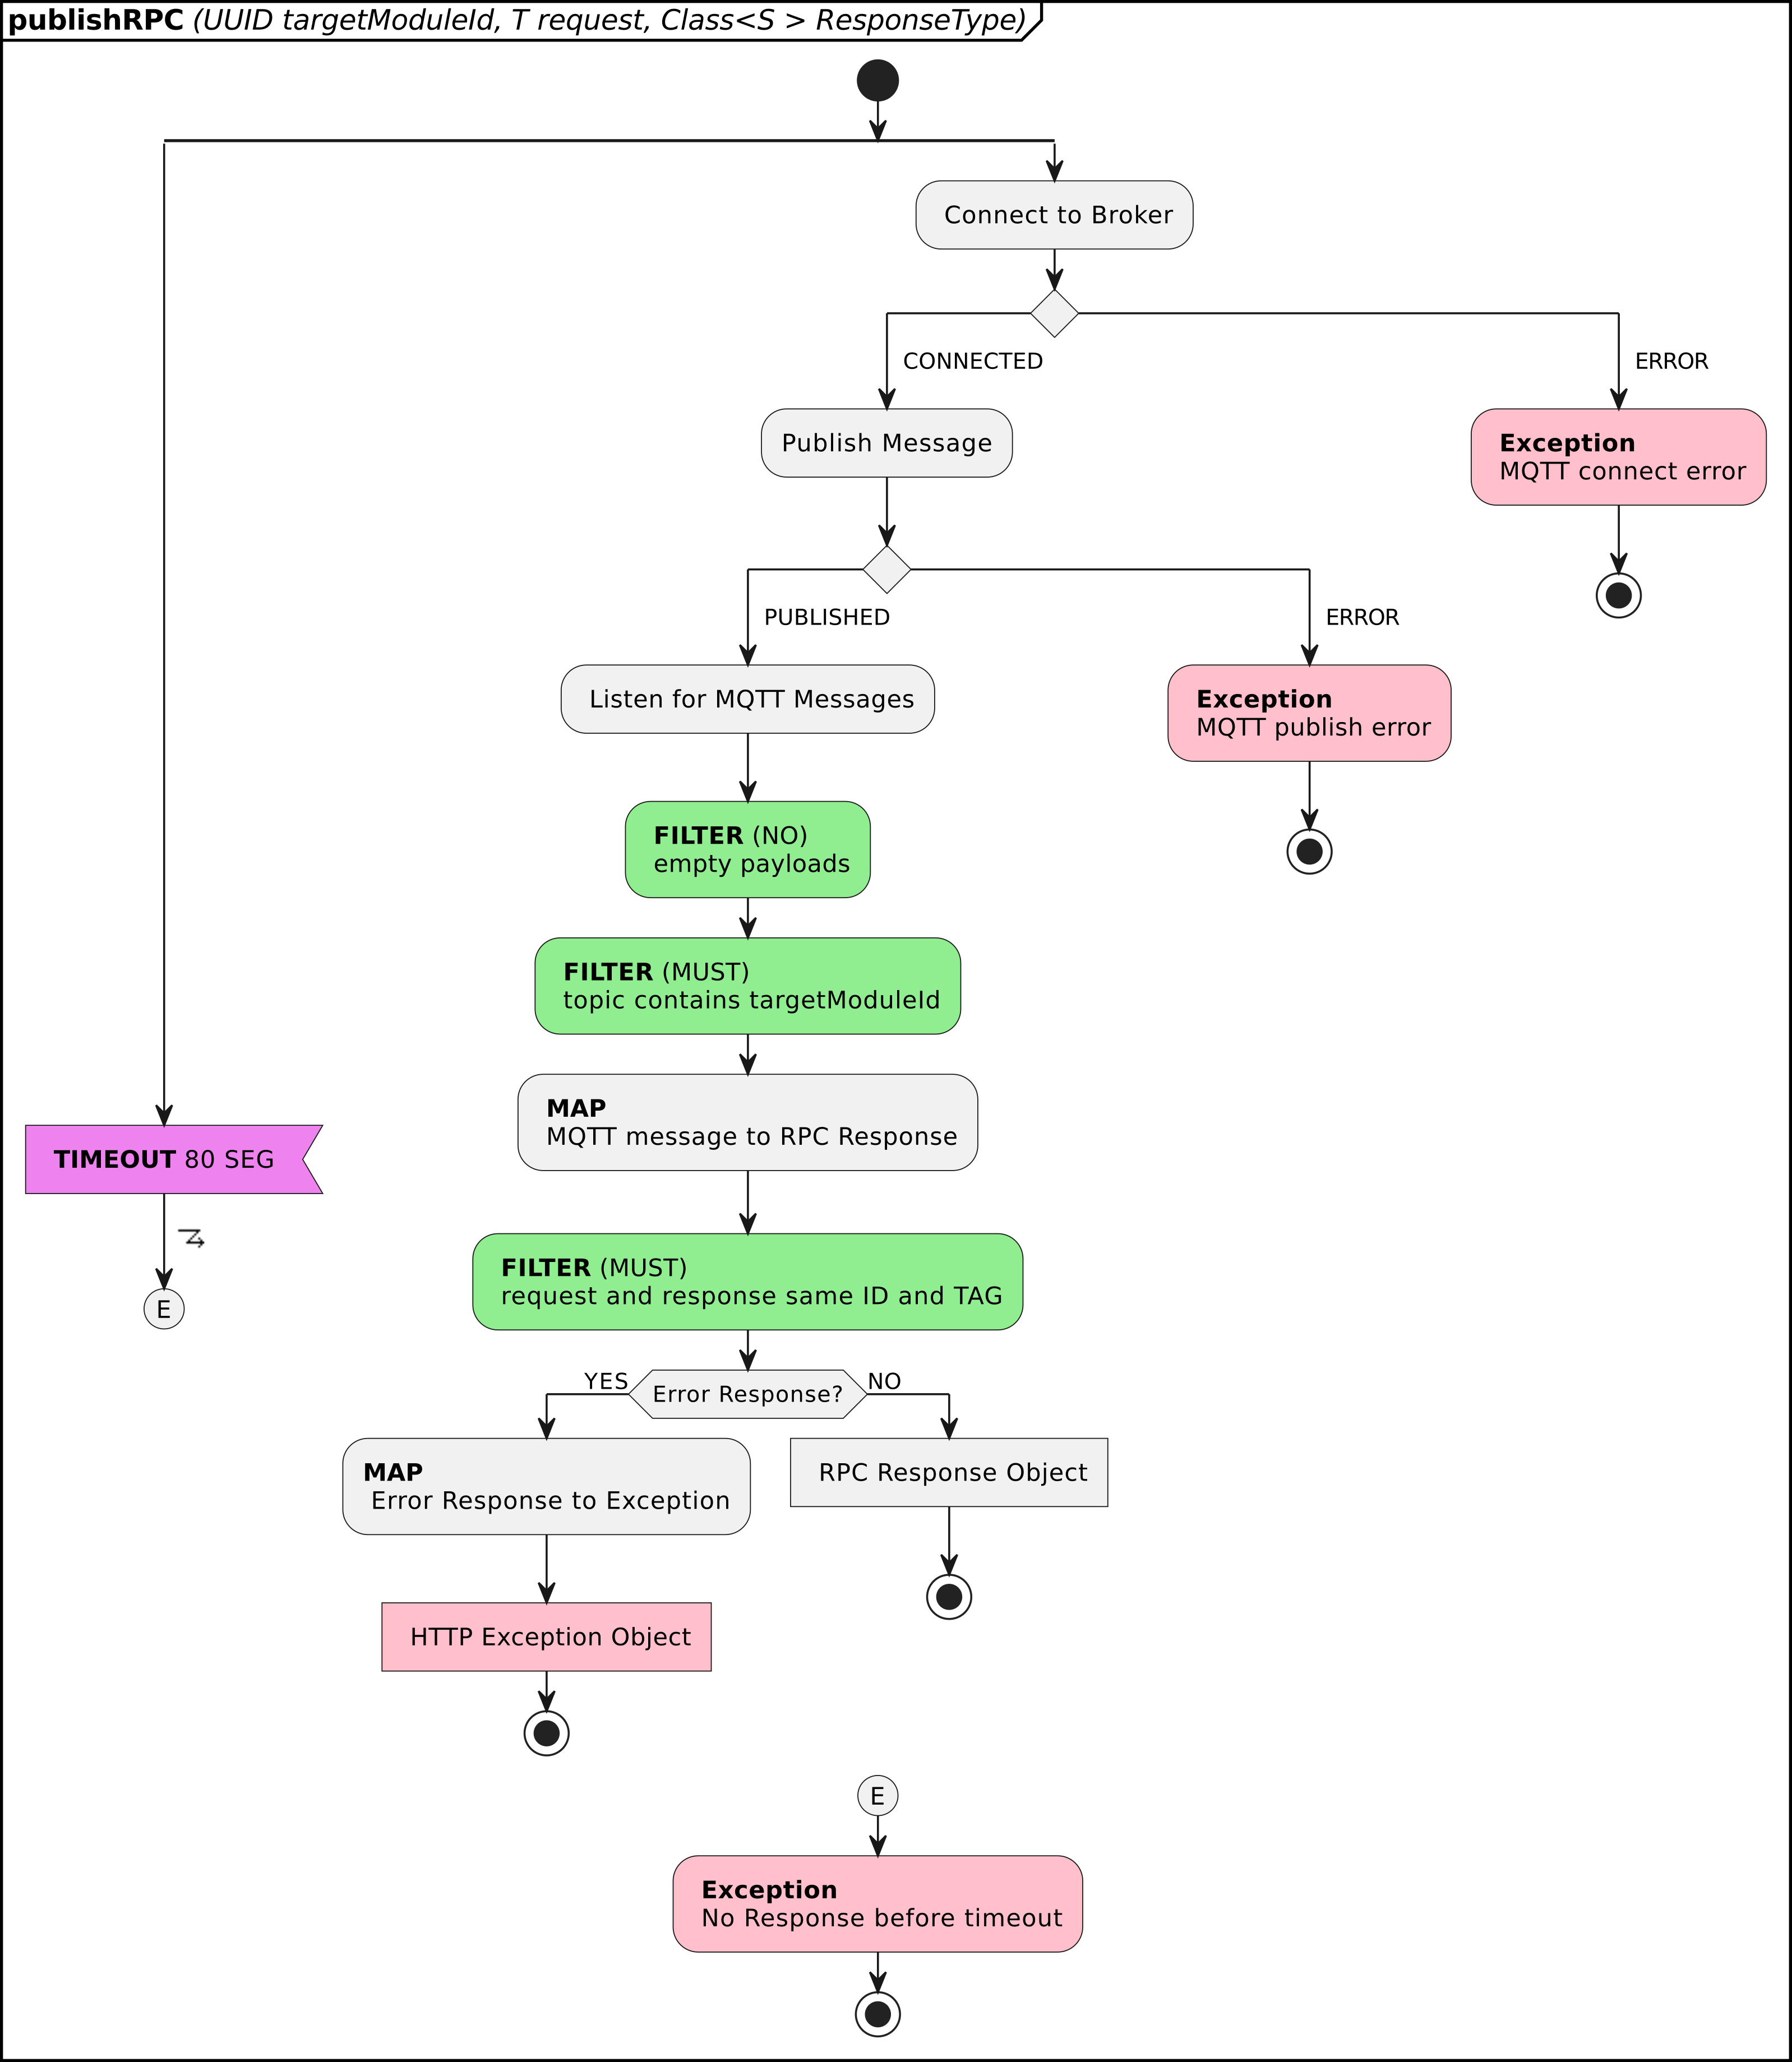
\includegraphics[width=0.9\textwidth]{Figures/iter3/ACT_publishRPC_ink.png}
	\rule{35em}{1pt}
	\caption[UML Diagram]{Diagrama de actividades del procedimiento de envío de una solicitud y recepción de la respuesta al momento de ejecutar un RPC.}
	\label{fig:act_publish_rpc}
\end{figure}

Existe un escenario que produce une excepción pero que no representa un fallo de la rutina sino que se genera a propósito como un mapeo de la respuesta de operación no exitosa enviada por el módulo y así conservar la compatibilidad con los casos de uso ya implementados.


\subsection{Selector de Canales}
Al introducir un nuevo canal de datos por el cual se pueden ejecutar los procedimientos remotos se hizo necesario incorporar una rutina que decida cuál es el canal apropiado para realizar la operación conforme a las condiciones de conexión del teléfono.
\subsubsection{Ejecutor}
Para resolver la tarea y teniendo en cuenta la similaridad de todos los métodos asociados a la ejecución de RPC, se optó por codificar una clase interna al repositorio denominada \texttt{RPCExecutor}. Esta clase se implementó utilizando tipos genéricos de Java ya que cada RPC utiliza objetos solicitud y respuesta de tipos únicos. \texttt{RPCExecutor} permite generalizar el modo de ejecución de los RPC de manera que el codigo en cada uno es equivalente.
Se declara un método de nombre \texttt{executeRPC} que hace uso del ejecutor para decidir la fuentes de datos primaria, con la que intentará ejecutar el procedimiento en caso de fallar intentará con la segunda si es que está disponible.
El orden de prioridad de estas fuentes de datos se determina en un método aparte denominado getDataSourceChoices. En la figura ~\ref{fig:act_choices} se muestra el algoritmo utilizado. El estado de conexión de teléfono se obtiene usando las APIs provista por el SDK de android.

\begin{figure}[htbp]
	\centering
	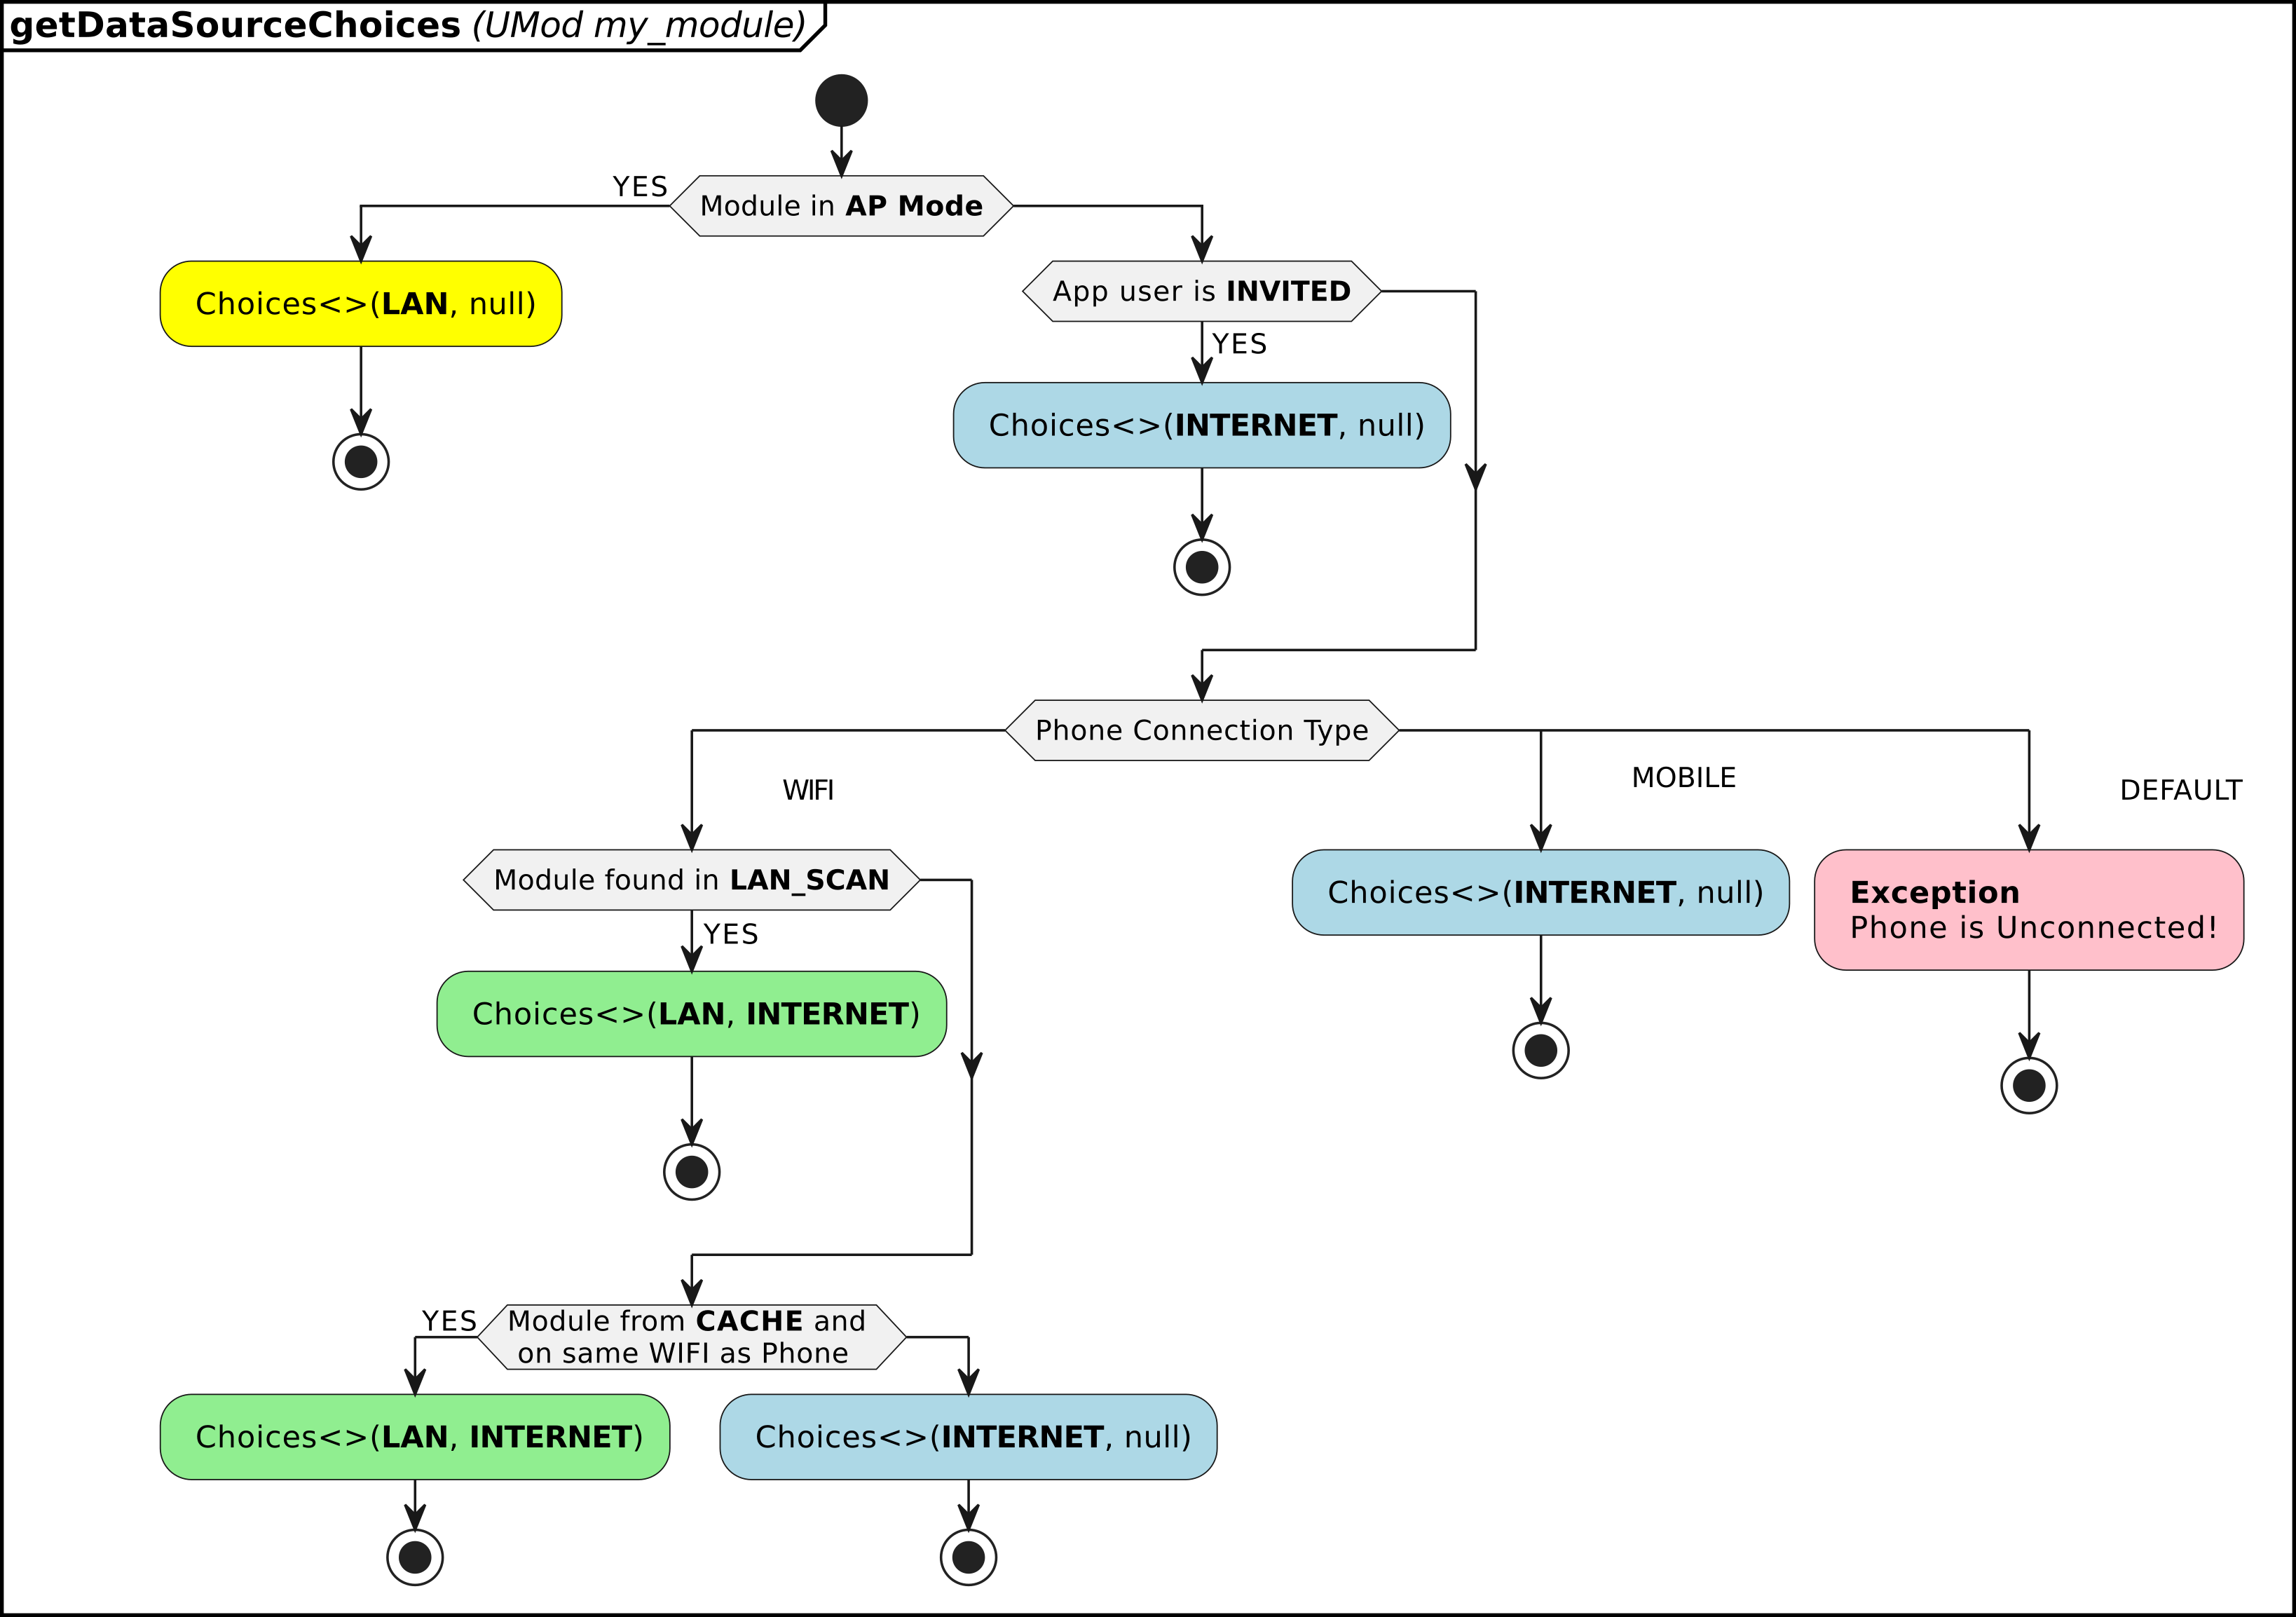
\includegraphics[width=0.9\textwidth]{Figures/iter3/ACT_choice_ink.png}
	\rule{35em}{1pt}
	\caption[UML Diagram]{Diagrama de actividades del procedimiento que determina el orden de prioridad de las fuentes de datos para la ejecucuín de RPC.}
	\label{fig:act_choices}
\end{figure}



\section{Casos de Uso Implementados}
Para la presente iteración se implementaron los siguientes casos de uso.
\begin{enumerate}
	\item Actualizar GATE-STATUS de los módulos.
	\item Activar Acceso Rápido.
	\item Actualizar Firmware
	\item Habilitar Módulo para Acceso Rápido.
	\item Accionar módulo cercano.
	\item Obtener módulos disponibles para acceso rápido.
	\item Desbloquear botón contra accionamiento accidental.
\end{enumerate}

A continuación se documentaran aquellos que presentan los escenarios más interesantes.

\subsection{Actualizar Firmware}
Este caso de uso es fundamental para garantizar la calidad del producto al proveer actualizaciones para el firmware del módulo.
El usuario administrador ingresa a la pantalla de configuración de un módulo, luego toca el botón asignado para esta operación, acepta el cartel de advertencia y espera hasta que concluya el procedimiento.
Como una nota al margen se menciona que por restricciones impuestas en el framework utilizado para programar el firmware del módulo la actualización OTA solo puede realizarse por el canal LAN y consiste de los siguientes pasos:
\begin{enumerate}
	\item El teléfono descarga un archivo .zip que corresponde a la nueva versión del firmware para el módulo.
	\item El teléfono envía este archivo al módulo mediante un POST HTTP multiparte a un endpoint predefinido que incluye el archivo del nuevo firmware y el valor \texttt{COMMIT\_TIMEOUT} que determina la cantidad de tiempo en segundos que esperará el módulo para que el usuario autorice la nueva versión luego de concluida la instalación y el reinicio exitoso.
	\item El teléfono espera que el módulo se reinicie y ejecuta el RPC GetSysInfo para corroborar la correcta versión del firmware recién instalado.
	\item COMMIT: El teléfono hace un POST HTTP a un endpoint predefinido para autorizar la actualización.
\end{enumerate} 

Este caso de uso utiliza hasta tres RPC en su ejecución y puede fallar en 8 escenarios distintos a saber:

\begin{enumerate}
	\item Error de comunicación con el módulo.
	\item Versión actual del firmware DESCONOCIDA.
	\item Actualización no necesaria.
	\item Error con la URL de descarga del archivo de firmware.
	\item El archivo descargado está vacío.
	\item Error de comunicación con el servidor.
	\item Error de versión después de actualizar.
	\item Error de COMMIT.
\end{enumerate} 

En el diagrama de la figura ~\ref{fig:act_ota} se puede observar el algoritmo implementado para este caso de uso.

\begin{figure}[htbp]
	\centering
	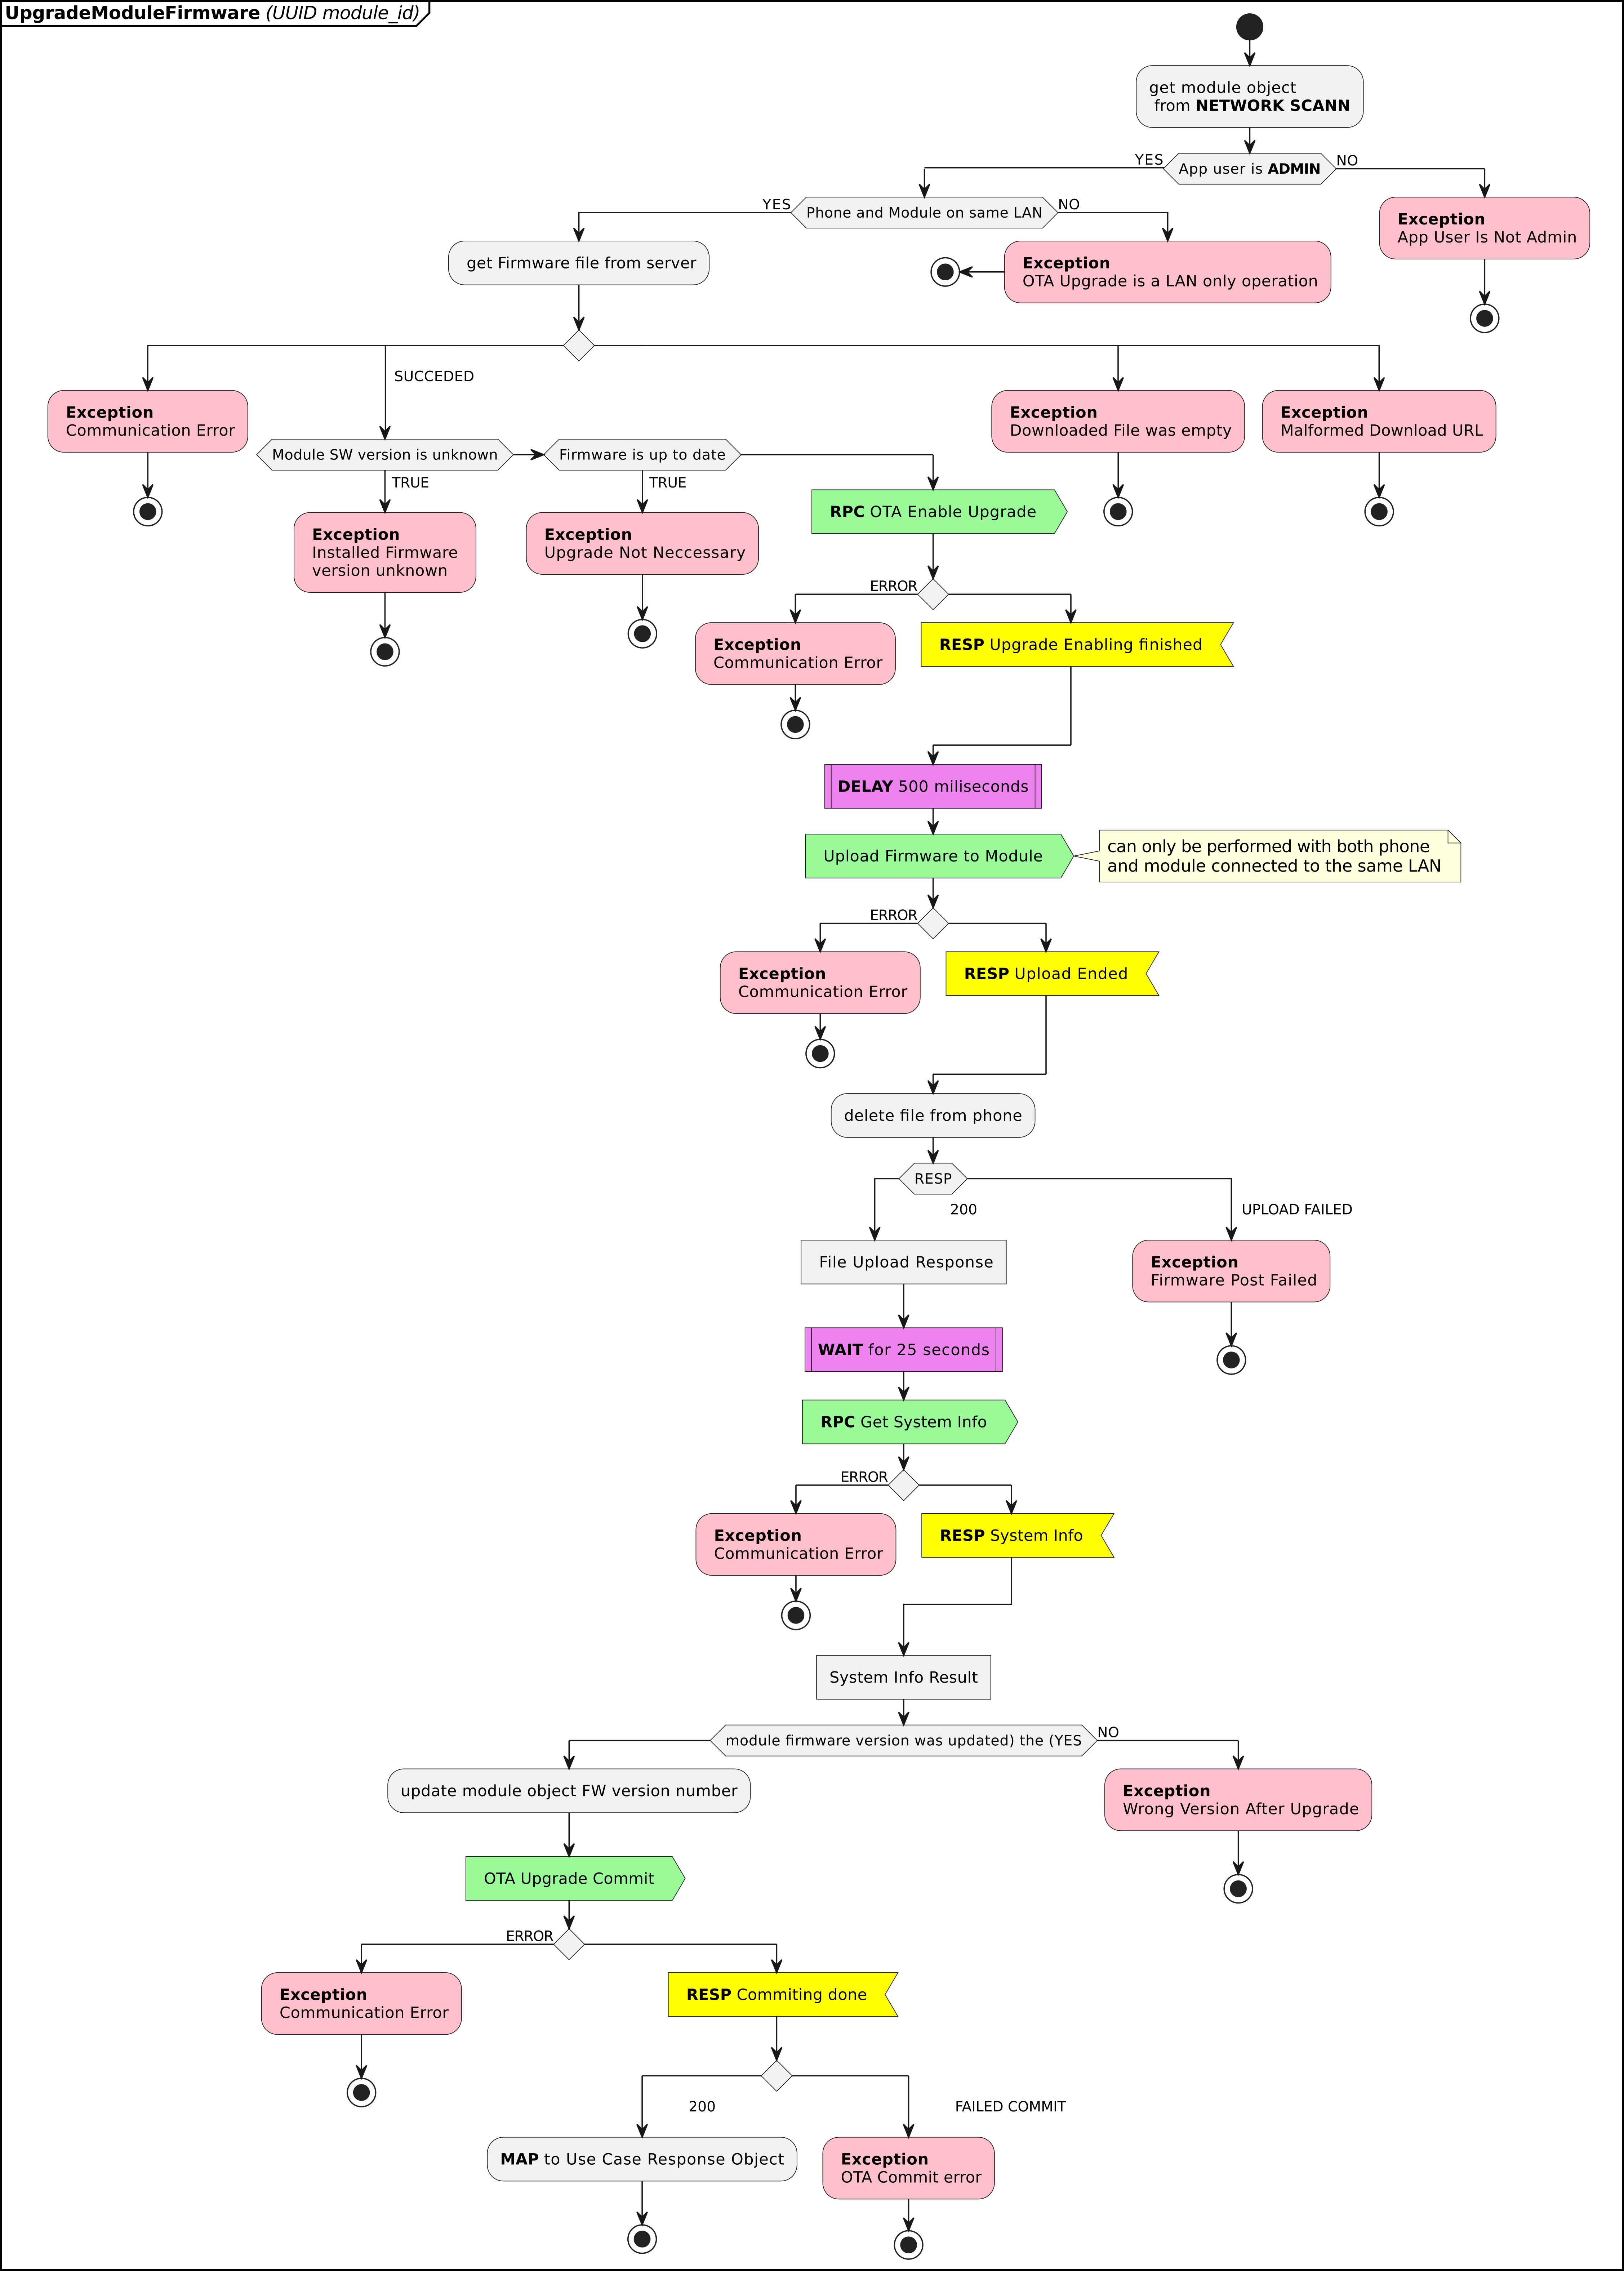
\includegraphics[width=\textwidth]{Figures/iter3/ACT_ota_ink.png}
	\rule{35em}{1pt}
	\caption[Class Diagram]{Diagrama de actividades de la implementación del caso de uso: Actualización de Firmware.}
	\label{fig:act_ota}
\end{figure}

\subsection{Obtener módulos disponibles para acceso rápido}
En la pantalla de bloqueo del teléfono sobre la notificación permanente el usuario presiona
el botón para refrescar los módulos disponibles para accionamiento rápido.
Este caso de uso obtiene la ubicación geográfica del teléfono que debe tener una precisión menor a 60 metros
y su última actualización no debe superar los 5 minutos.
Una vez conocida la posición geográfica del teléfono buscará todos los módulos que cumplan las siguientes condiciones:
\begin{itemize}
	\item El modulo debe estar en STATION\_MODE.
	\item El usuario de la app debe estar autorizado.
	\item El modulo debe tener habilitado el control rápido.
	\item El módulo debe encontrarse a menos de 320 metros de distancia.
\end{itemize}
Este caso de uso no realiza llamadas a RPCs y puede fallar en 8 escenarios.
En la figura ~\ref{fig:act_notif_modules} se puede observar el diagrama de actividades de la implementación del caso de uso.

\begin{figure}[htbp]
	\centering
	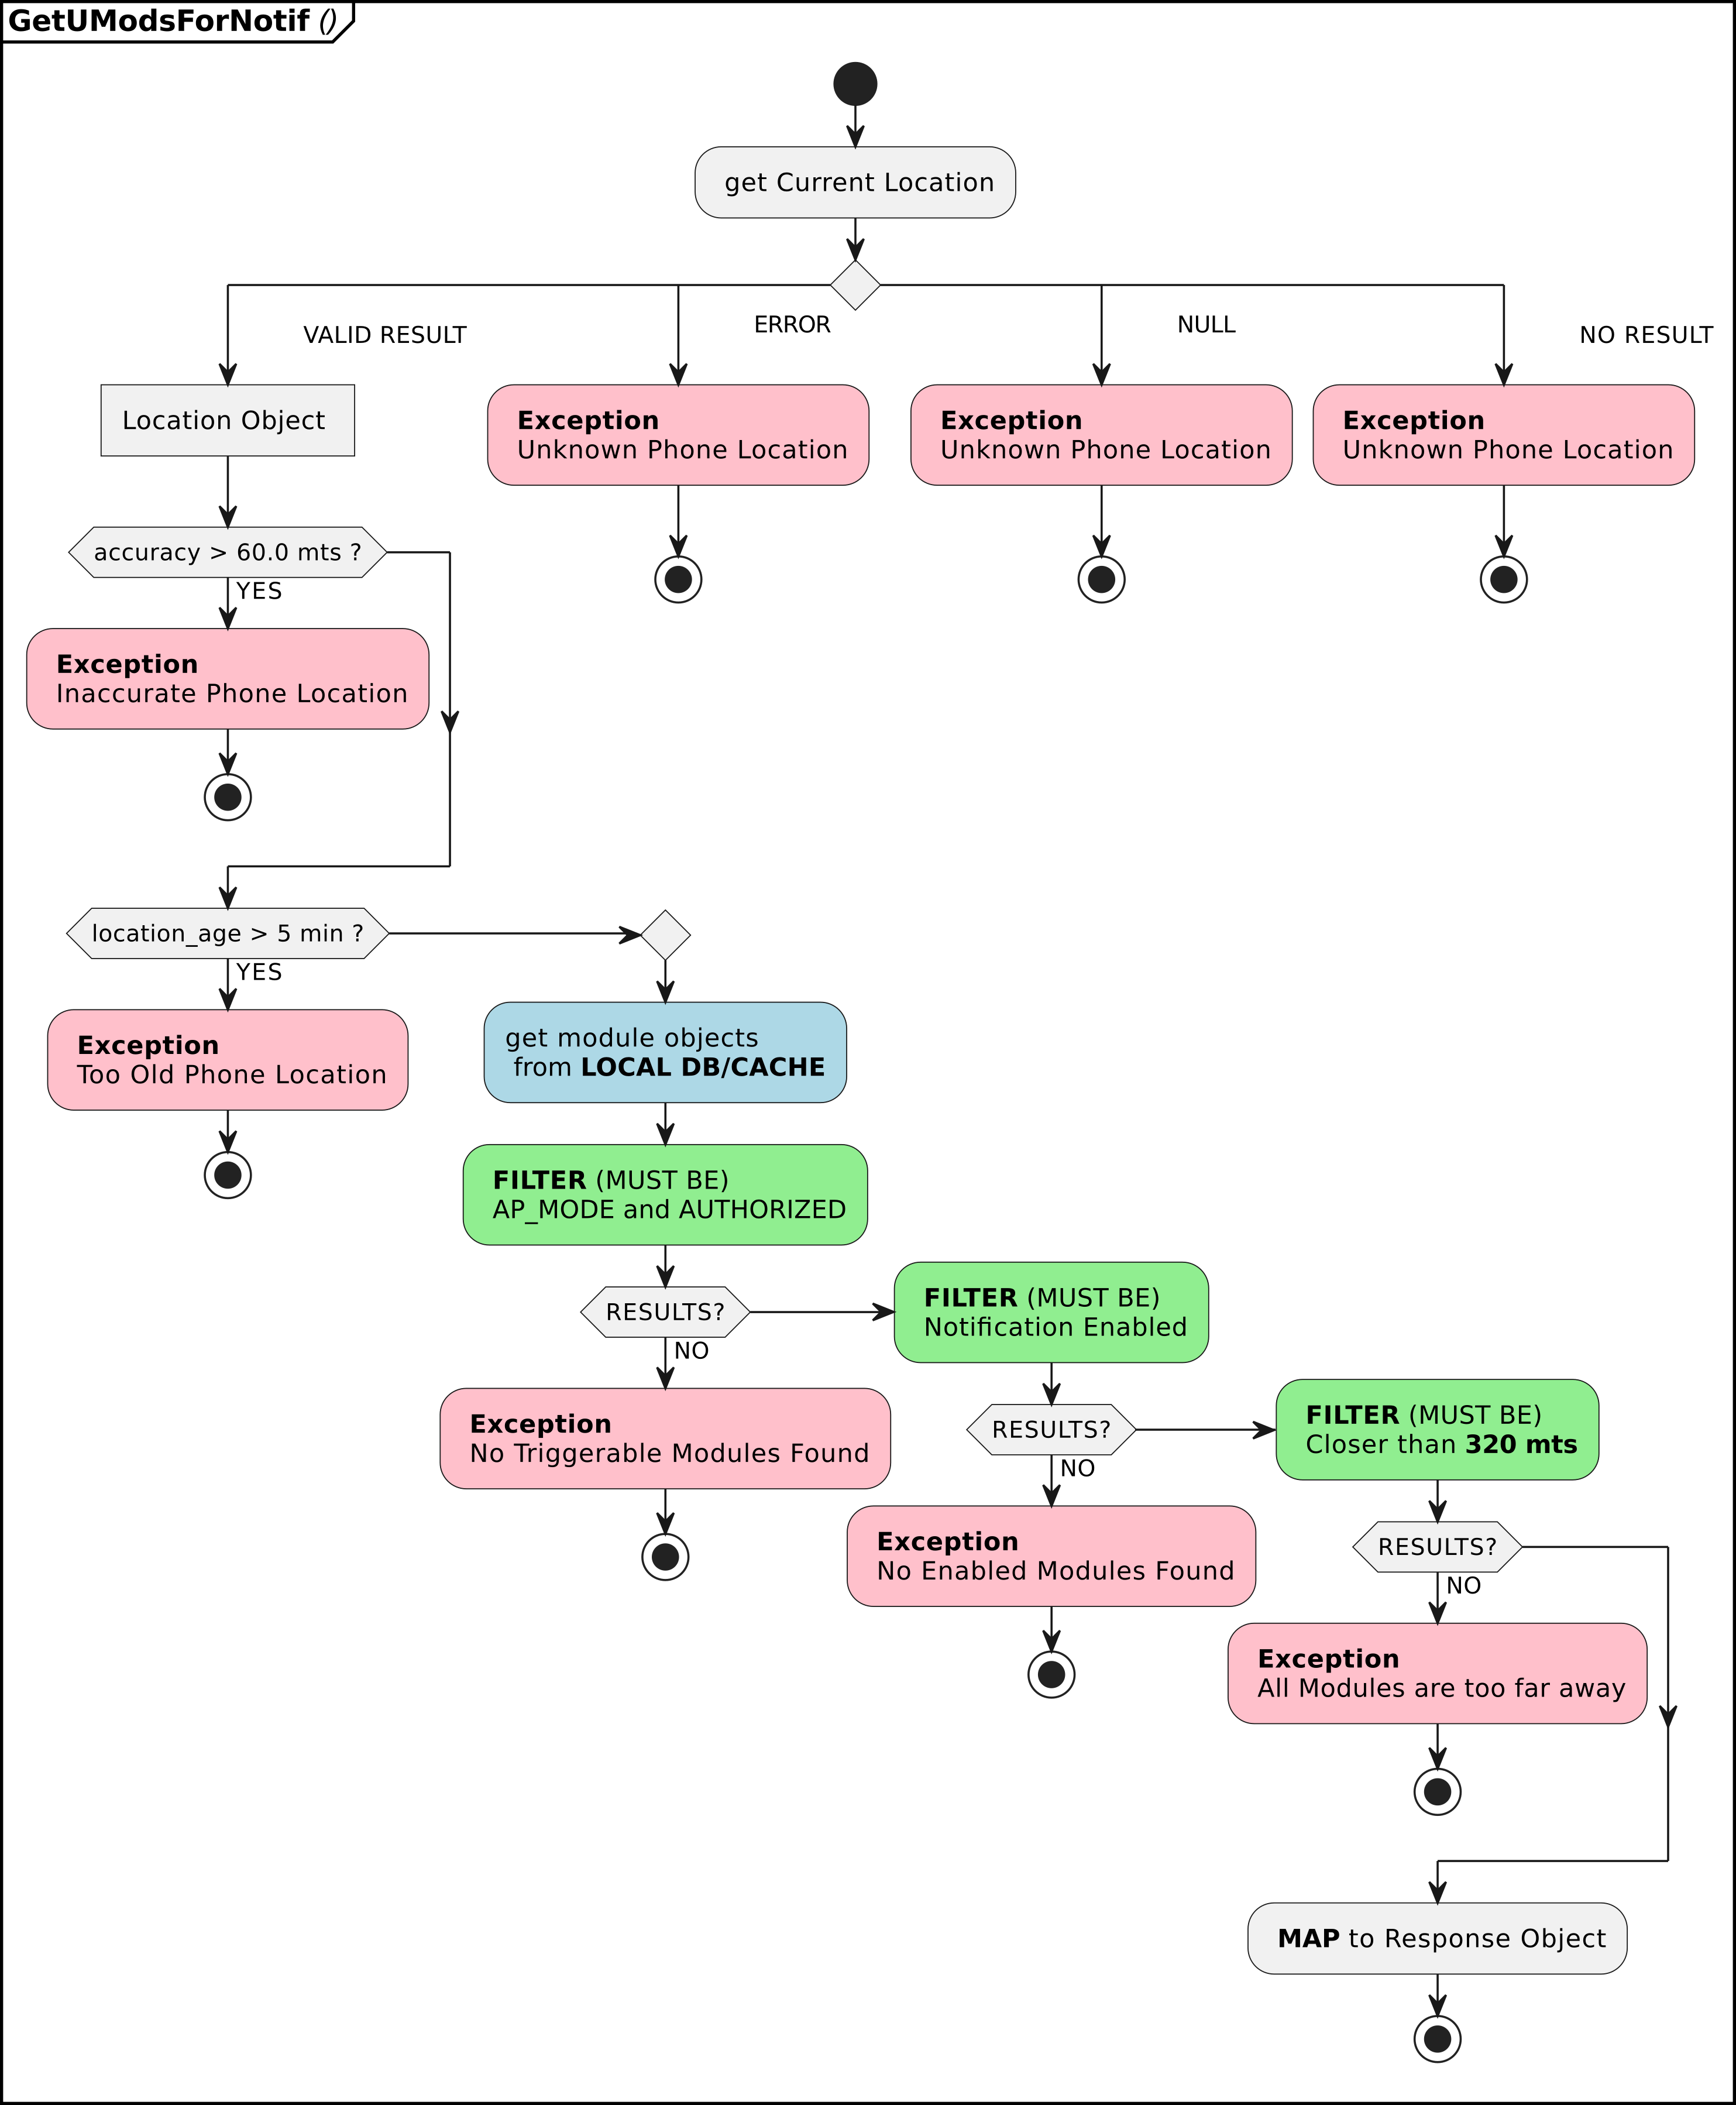
\includegraphics[width=0.8\textwidth]{Figures/iter3/ACT_getModsNotif.png}
	\rule{35em}{1pt}
	\caption[Class Diagram]{Diagrama de actividades de la implementación del caso de uso: Obtener módulos disponibles para acceso rápido.}
	\label{fig:act_notif_modules}
\end{figure}

